\documentclass[twoside,english]{uiofysmaster}

%\bibliography{references}

\author{Fredrik Wilhelm Holmen}
\title{Master thesis Wilhelm Coupled Cluster}
\date{Autumn 2015}

\begin{document}
% set space around equations
\setlength{\belowdisplayskip}{12pt} \setlength{\belowdisplayshortskip}{12pt}
\setlength{\abovedisplayskip}{12pt} \setlength{\abovedisplayshortskip}{12pt}


\maketitle

\begin{abstract}
  This is an abstract text.
\end{abstract}

\begin{dedication}
  To someone
  \\\vspace{12pt}
  This is a dedication to my cat.
\end{dedication}

\begin{acknowledgements}
  I acknowledge my acknowledgements.
\end{acknowledgements}

\tableofcontents



\begin{chapter}{Introduction}
  This is a very nice introduction to my myster thesis.
  or ..
  lol
\end{chapter}





\begin{chapter}{Quantum Mechanics}
 
 \begin{section}{Postulates}
 	
 \end{section}

 \begin{section}{Hermitian Operators}
 	
 \end{section}

 \begin{section}{Pauli's Exclusion Principle}
 	
 \end{section}

 \begin{section}{The Variational Principle}
 	
 \end{section}

 \begin{section}{Slater Determinant}
 	A system composed of a nuclei and electrons moving in accordance to the forces of electromagnetic attraction can be described by assigning each electron
	a wave function 
	\begin{align}
		\phi_i(\mathbf{x}_i)
	\end{align}
	Where $\mathbf{x}_i$ is the position vector for the electron i. Describing a system of many electrons can be done writing a Slater Determinant
	\begin{align}
		\ket{\Phi_0} = \frac{1}{ \sqrt{N!} } \left|\begin{matrix}
			\phi_1(\mathbf{x}_1) & \phi_2(\mathbf{x}_1) & ... & \phi_N(\mathbf{x}_1) \\
			\phi_1(\mathbf{x}_2) & \phi_2(\mathbf{x}_2) & ... & \phi_N(\mathbf{x}_2) \\
			... & & & \\
			\phi_1(\mathbf{x}_N) & \phi_2(\mathbf{x}_N) & ... & \phi_N(\mathbf{x}_N) 
		\end{matrix} \right|
	\end{align}
	This way of writing the many-body wave function will represent linear a combination of products of the one-body wave functions $\phi_i$'s and all the electronic coordinates
	$\mathbf{x}_i$ distributed among them in all possible ways. Exchanging two lines will change the sign such that the Slater Determinant will respect the anti-symmetry 
	requirement. \par
	We can choose the one-body wave functions that is most rewarding the specified system. When calculating on electrons moving with respect to a nuclei, one can choose the wave
	functions to be the 1s, 2s, 2p, .. orbitals. This representation will not, however, take into account the Coulombic repulsion between two electrons and will only be an 
	approximation to the true wavefunction, $\ket{\Psi}$.
 \end{section}

\end{chapter}





\begin{chapter}{Second Quantization}
 Second quantization is a new method of representing states and operators. 
 \begin{section}{Annihilation and Creation operators}
 	We introduce a new way of writing states using the mathematical technique known as second quantization. The main goal is to treat states without paying attention
  	to individual particle coordinates. We represent the empty space with the symbol for vacuum
  	\begin{align}
  		\ket{0}
  	\end{align}
  	To represent a state, we use a creation operator to add the state to the vacuum.
  	\begin{align}
  		\hat a_i^{\dagger} \ket{0} = \ket{\phi_i}
  	\end{align}
  	And the annihilation operator will remove the particle again. 
  	\begin{align}
  		\hat a_i \ket{\phi_i} = \ket{0}
  	\end{align}
  	Trying to add a new particle to an already filled state and removing an unoccupied state results in zero.
  	\begin{align}
  		\hat a_i^{\dagger} \ket{\phi_i} = 0 \;\;\;\;\; \hat a_i \ket{0} = 0
  	\end{align}
  	We can now write the Slater determinant as a chain of creation operators
  	\begin{align}
  		\hat a_1^{\dagger} \hat a_2^{\dagger}... \hat a_N^{\dagger} \ket{0}
  	\end{align}
  	Permutations of the operators introduces a sign-change, which is equivalent to interchanging rows in the determinant. This 
  	\begin{align}
  		\hat a_1^{\dagger} \hat a_2^{\dagger} \ket{0} = \ket{\phi_1 \phi_2} = -\ket{\phi_2 \phi_1} = -\hat a_2^{\dagger} \hat a_1^{\dagger} \ket{0}
  	\end{align}
  	So we can see that the second quantization respects the antisymmetrization condition. Thus, these operators follow the anti commutation relations
  	\begin{align}
  		\{ \hat a_i^{\dagger} \hat a_j \} = \delta_{ij} \;\;\;\;\; \{ \hat a^{\dagger}_i \hat a^{\dagger}_j \} = 0 \;\;\;\;\; \{ \hat a_i \hat a_j \} = 0
  	\end{align}
  	Where $\delta_{ij}$ is the Kronecher delta. 
 \end{section}

 \begin{section}{Representation of Operators}
 	
 \end{section}

 \begin{section}{Fermi Vacuum}
 	
 \end{section}

 \begin{section}{Normal Ordering and Wick's Theorem}
 	
 \end{section}

 \begin{section}{Partitioning the Hamiltonian}
 	
 \end{section}
 
\end{chapter}




\begin{chapter}{Many-Body Methods}
	We have already justified the use of a Slater Determinant to describe the first approximation of the full wave function, $\ket{\Psi}$. Where
	\begin{align}
		\ket{\Psi} \approx \ket{\Phi_0} = 	\frac{1}{ \sqrt{N!} } \left|\begin{matrix}
			\phi_1(\mathbf{x}_1) & \phi_2(\mathbf{x}_1) & ... & \phi_N(\mathbf{x}_1) \\
			\phi_1(\mathbf{x}_2) & \phi_2(\mathbf{x}_2) & ... & \phi_N(\mathbf{x}_2) \\
			... & & & \\
			\phi_1(\mathbf{x}_N) & \phi_2(\mathbf{x}_N) & ... & \phi_N(\mathbf{x}_N) 
		\end{matrix} \right|
	\end{align}	
	This first representation fails to account for the Coulombic interrraction between the electrons, and we need higher-order approximations on top 
	of the Slater Determinant to improve our results. \par
	This chapter will look at three methods, namely the Configuration interraction, Many-body Perturbation theory and Hartree-Fock approximations. The
	Master thesis is on Coupled Cluster theory, and that will be more elaborately explained in it's own chapter. It is useful to benchmark Coupled Cluster 
	with similar many-body method. 

 \begin{section}{Configuration Interraction}
 		We can write the configuration interaction wavefunction as 
  	\begin{align}
  		\ket{\Psi_{CI}} = (1 + \hat C) \ket{\Phi_0} 
   	\end{align}
  	\begin{align}
  		\hat C = \hat C_1 + \hat C_2 + ... =  \sum_{ia} c_i^a a_a^{\dagger} a_i + \frac{1}{4} \sum_{ijab} c_{ij}^{ab} a_a^{\dagger} a_b^{\dagger} a_j a_i + ...
   	\end{align}
 \end{section}	

 \begin{section}{Many-body Perturbation Theory}
 	
 \end{section}

 \begin{section}{Hartree-Fock approximations}
 	
 \end{section}

\end{chapter}




\begin{chapter}{Coupled-Cluster Theory}
 	In Coupled Cluster theory, the ansatz we make is to make an expansion in the wave function
 	\begin{align}
 		\ket{\Psi} \approx e^{\hat T} \ket{\Psi_0}
  	\end{align}
  	The operator $\hat T$ is a linear combination of the cluster operators
  	\begin{align}
  		\hat T = \hat T_1 + \hat T_2 + \hat T_3 + ... + \hat T_N
  	\end{align}
  	Where the operators represent
  	\begin{align}
  		T_1 &= \sum_{ia} t_i^a \hat a_a^{\dagger} \hat a_i \\
  		T_2 &= \frac{1}{2} \sum_{ijab} t_{ij}^{ab} \hat a_a^{\dagger}\hat a_b^{\dagger} \hat a_j \hat a_i \\
  		T_2 &= \left(\frac{1}{n!}\right)^2 \sum_{ij..ab..}^n t_{ij..n}^{ab..n} \hat a_a^{\dagger}\hat a_b^{\dagger} ...\hat a_n^{\dagger} \hat a_n ... \hat a_j \hat a_i \\
  	\end{align}

  	We can write the configuration interaction wavefunction as 
  	\begin{align}
  		\ket{\Psi_{CI}} = (1 + \hat C) \ket{\Phi_0} 
   	\end{align}
  	\begin{align}
  		\hat C = \hat C_1 + \hat C_2 + ... =  \sum_{ia} c_i^a a_a^{\dagger} a_i + \frac{1}{4} \sum_{ijab} c_{ij}^{ab} a_a^{\dagger} a_b^{\dagger} a_j a_i + ...
   	\end{align}
   	Comparing this linear expansion to the exponential expansion from Coupled Cluster, we can see that
   	\begin{align}
   		\hat C_2 = \hat T_2 + \frac{1}{2} T_1^2
   	\end{align}
   	Where we can see that even if we truncate Configuration Interaction and Coupled Cluster at the same level, there are more \textit{disconnected} wave function contributions (REFERENCE page 17 IN C\&S) in the Coupled Cluster theory. Both the Coupled Cluster and Configuration Interaction theory provides the exact energy by including the operators to infinite order, i.e. no truncation. 

  	\begin{section}{Size Extensivity}
  		It can be important to have a wave function that scales with size. Imagine a two particles, $X$ and $Y$ with infinity separation, they do not interact. This means we should be able to write the total energy as
  		\begin{align}
  			E = E_X + E_Y
  		\end{align}
  		Doing Coupled Cluster
  		\begin{align}
  			\hat T = \hat T_X + \hat T_Y 
  		\end{align}
  		\begin{align}
  			\ket{\Psi}_{CC} = e^{\hat T_X + \hat T_Y} \ket{\Phi_0} = e^{\hat T_X} e^{\hat T_Y} \ket{\Psi_0}
  		\end{align}
  		Since we can write the reference state as a product of the two seperated parts, we are able to write
  		\begin{align}
  			E_{CC} = E_{CC}^X + E_{CC}^Y
  		\end{align}
  		This means Coupled Cluster is size extensive, contrary to the Configuration Interaction. 
  	\end{section}

\end{chapter}




\begin{chapter}{The Pairing Model}
	The first system I look at is the pairing model. The pairing model has four energy levels with degeneracy two, one for positive and negative spins. I have 
	used a system consisting of four electrons filling up the four lower-most states up to the Fermi level. 
	\begin{figure}[h]
		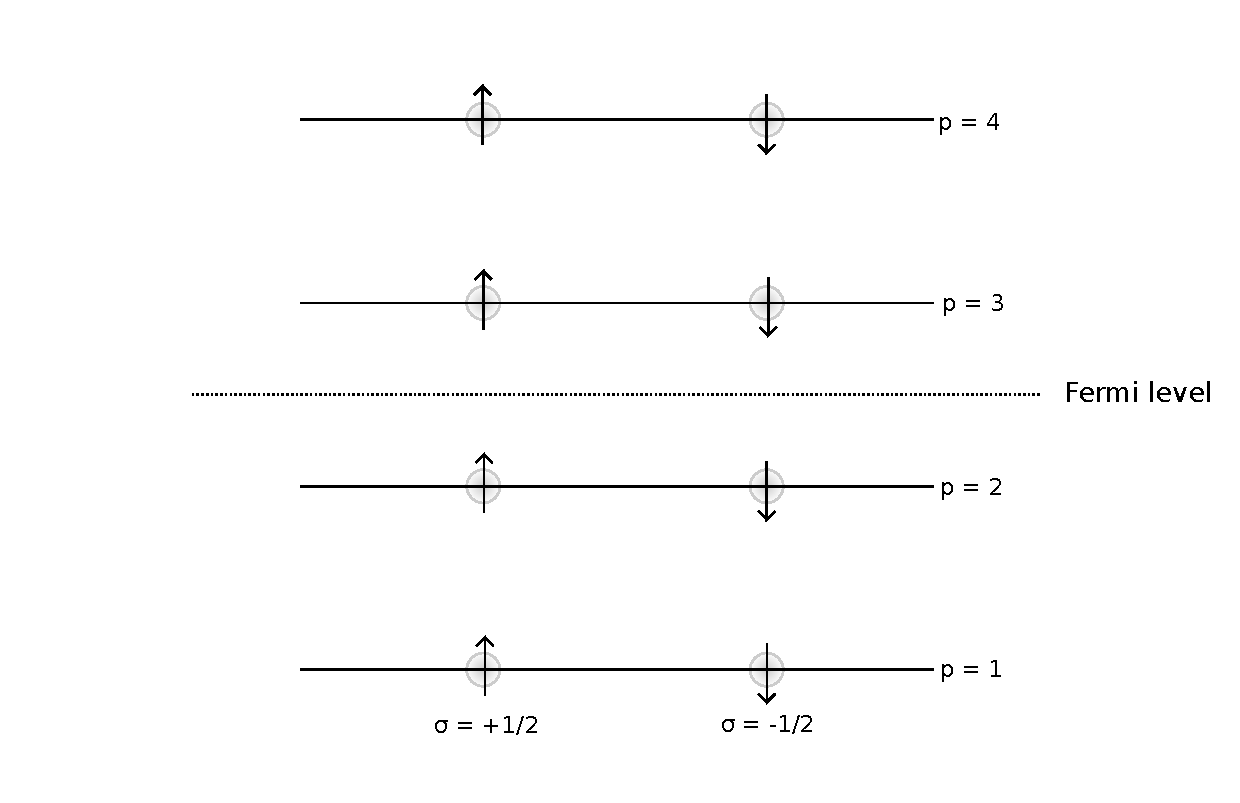
\includegraphics[width=\textwidth]{Figures/Pairing_model.pdf}
		\label{PairingModel_1}
		\caption{A figure depicting a 4 particles-4 holes state. The system consists of occupied particle states below the Fermi level and unoccupied hole states above Fermi level.}
	\end{figure}
	
	\begin{section}{The Hamiltonian}
		We limit ourselves to a two-body interaction, writing the Hamiltonian as
		\begin{align}
			\hat H = \sum_{\alpha \beta} \left< \alpha \right| \hat h_0 \left| \beta \right> \hat a_{\alpha}^{\dagger} \hat a_{\beta} 
			        + \frac{1}{4} \sum_{\alpha \beta \gamma \delta} \left< \alpha \beta \middle| \hat v_0 \middle| \gamma \delta \right> \hat a_{\alpha}^{\dagger} \hat a_{\beta}^{\dagger} \hat a_{\delta} \hat a_{\gamma}
		\end{align}
		We use the complete basis $\left| \alpha \right>$ and define the set as eigenvalues of the one-body operator, $\hat h_0$. 
		
		The system does require that the total spin is equal to $0$. In addition we will not allow spin pairs to be broken, i.e.\  singly excitated states are not allowed. 
		\begin{align}
			\left| \Psi_i^a \right> = 0 
		\end{align}	
		We introduce the double creation and annihilation operator. 
		\begin{align}
			\hat P_{pq}^{\dagger} = \hat a_{p \sigma}^{\dagger} \hat a_{p -\sigma}^{\dagger}
		\end{align}
		\begin{align}
			\hat P_{pq} =  a_{q \sigma} a_{q -\sigma}
		\end{align}

		We can rewrite the Hamiltonian as an unperterturbed part and a perturbation
		\begin{align}
			\hat H = \hat H_0 + \hat V
		\end{align}
		\begin{align}
			\hat H_0 = \xi \sum_{p \sigma} (p-1) \hat a_{p \sigma}^{\dagger} \hat a_{p \sigma}
		\end{align}
		\begin{align}
			\hat V = - \frac{1}{2}g \sum_{pq} \hat a_{p +}^{\dagger} \hat a_{p-}^{\dagger} \hat a_{q-} \hat a_{q+}
		\end{align}
		The value of $\xi$ determines the spacing between the energy levels, which I have set to $1$. This will not impact the insight attained solving this system. $p$ and $q$ determines the energy level. $\sigma$ is the spin, with value either $+\frac{1}{2}$ or $-\frac{1}{2}$. Both the unperturbed and perturbed Hamiltonian keeps total spin at $0$
	\end{section}
	\begin{section}{Configuration Interaction theory}
		This system is a good way to benchmark various methods as we can compute the exact solution using Full Configuration Interaction. 
		\begin{figure}
			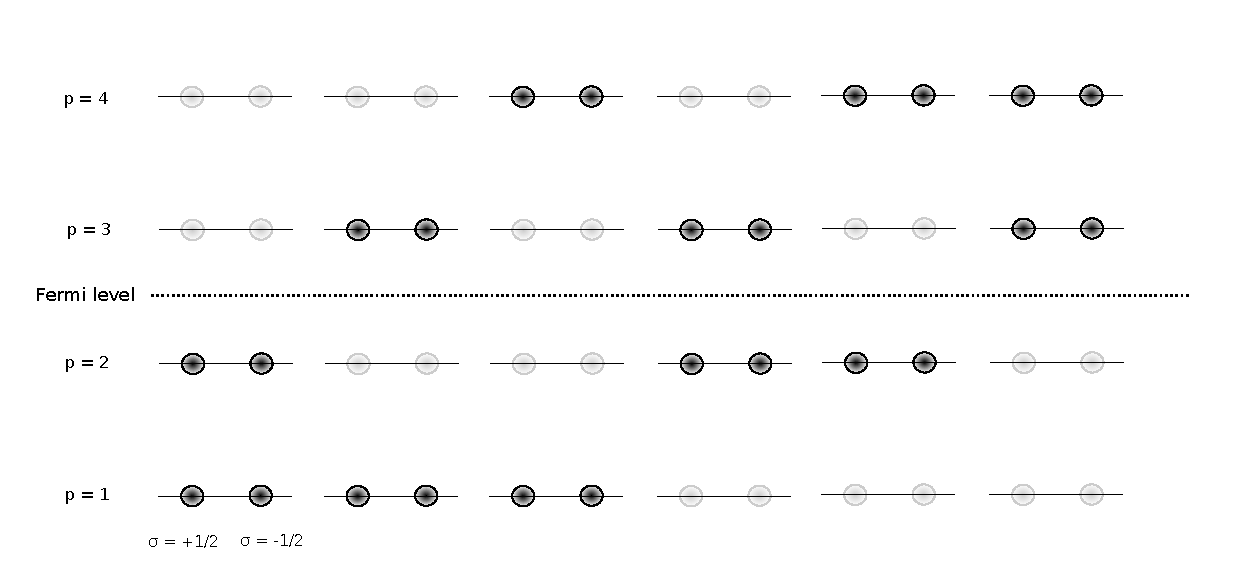
\includegraphics[width=1.1\linewidth]{Figures/Pairing_model2.pdf}
			\label{PairingModel_2}
			\caption{Configuration space for given pairing model showing all possible distributions of electrons}
		\end{figure}

		
	\end{section}

\end{chapter}




\begin{chapter}{Infinite Matter}
	A study of infinite matter is the most comprehensible way of studying nuclear material. This thesis will study the infinite electron gas before the final study of nuclear material. This is done because of pedagogical reasons and because the electron gas has closed form solutions that provide important benchmarking for the code. 
	\begin{section}{The Infinate Electron Gas}
		The infinite electron gas gives a good approximation to valence electrons in metal. The gas consist only of interacting electrons with a uniform background of charged ions. The whole system is charge neutral. We assume a cubic box, length $L$ and volume $\Omega = L^3$, with $N_e$ as the number of electrons with a charge density $\rho = N_e / \Omega$.

		We regard the system as homogenic, using the free particle normalized wave function
		\begin{align}
		 	\psi_{\vec k \sigma} (\vec r) = \frac{1}{\sqrt{\Omega}} e^{i \vec k \vec r} \xi_{\sigma}
		 \end{align}
		 Where $\vec k$ is the wave number and $\xi_{\sigma}$ is a spin function. 
		 \begin{align}
		 	\xi_{+\frac{1}{2}} = \left( \begin{matrix} 1 \\ 0 \end{matrix} \right) \:\;\:\; \xi_{-\frac{1}{2}} = \left( \begin{matrix} 0 \\ 1 \end{matrix} \right)
		 \end{align}
		 Assuming periodic boundary conditions, we acquire the following wave numbers
		 \begin{align}
		 	k_i = \frac{2\pi n_i}{L} \:\:\:\;\; i = x,y,z \;\;\:\:\: n_i = 0, \pm 1, \pm 2, ...
		 \end{align}
		 The electrons interact with the sentral symmetric Colomb potential, $\hat V(\vec r_1, \vec r_2)$ depending only on the distance $\left| \vec r_1 - \vec r_2 \right|$. 

		 The Hamiltonian for infinite electron gas is
		 \begin{align}
		 	\hat H = \hat T + \hat V
		 \end{align}
		 Where we have the kinetic energy, $hat T$ as
		 \begin{align}
		 	\hat T = \sum_p \frac{\hbar ^2 k^2}{2m} a_{k \sigma}^{\dagger} a_{k \sigma}
		 \end{align}


		 
	\end{section}
\end{chapter}




\begin{chapter}{Implementation}
	
\end{chapter}




\begin{chapter}{Results}
	
\end{chapter}




\begin{chapter}{Appendix}
	
\end{chapter}



\end{document}